%
% programming.tex
%
% Copyright (C) 2023 UFSC.
%
% DOCUMENTATION-TEMPLATE
%
% This work is licensed under the Creative Commons Attribution-ShareAlike 4.0
% International License. To view a copy of this license,
% visit http://creativecommons.org/licenses/by-sa/4.0/.
%

\chapter{FPGA's Output GPIO Pinout}

    \section{LEDs}
        There are 27 user-controllable LEDs on the DE2i-150 board. Eighteen red LEDs are situated above
        the 18 Slide switches, and eight green LEDs are found above the push-button switches (the 9th
        green LED is in the middle of the 7-segment displays). We are going to use 8 red LEDs and 8 green LEDs. \autoref{tab:ledg} and \autoref{tab:ledr} shows the assignments of FPGA pins to the LEDG and LEDR. 
        
    \section{7-segment Display}
        The DE2i-150 Board has eight 7-segment displays.
        Each segment in a display is identified by an index from 0 to 6, with the positions given in \autoref{figure:hex}. \autoref{tab:hex} shows the assignments of FPGA pins to the 7-segment displays.
        
            \begin{figure}[!ht]
                \begin{center}
                    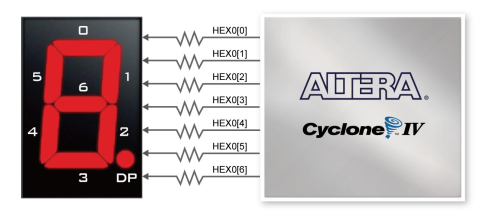
\includegraphics[width= 0.7\textwidth]{figures/chap2/hex.png}
                    \caption{\label{figure:hex} Connections between the 7-segment display HEX0 and Cyclone IV GX FPGA}
                \end{center}
            \end{figure}
    
    \section{LCD Display}
        The LCD module has built-in fonts and can be used to display text by sending appropriate
        commands to the display controller called HD44780. \autoref{tab:lcd} and \autoref{figure:lcd} shows the assignments of FPGA pins to the LCD.
        
        \newpage
            
            \begin{figure}[!ht]
                \begin{center}
                    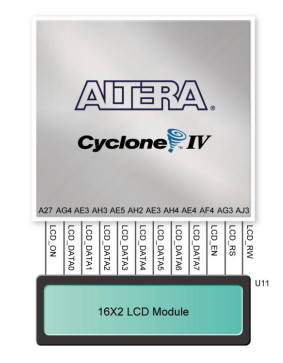
\includegraphics[width= 0.4\textwidth]{figures/chap2/lcd.png}
                    \caption{\label{figure:lcd} Connections between the LCD module and Cyclone IV GX FPGA}
                \end{center}
            \end{figure}
    
%%%%%%%%%%%%%%%%%%%%%%%%%%%%%%%%%%%%%%%%%%%%%%%%%%%%%%%%%%%%%%%%%%%%%%%%%%%%%%%%%%%%%%%%%%%%%%%%%%%%%%%%%

\chapter{Recording to the FPGA's Internal Memory} 

    In order for the Hardware described in VHDL to remain permanently in the FPGA, it is necessary to record it in the internal memory.
    
    \section {Step by step to record in internal memory}
    
        1. Open the .sof to .pof converter (programming object file)
        
        Path: In the File tab of Quartus II, open Convert Programming Files (Figure \ref{f1}).
        
            \begin{figure}[!ht]
                \begin{center}
                
                    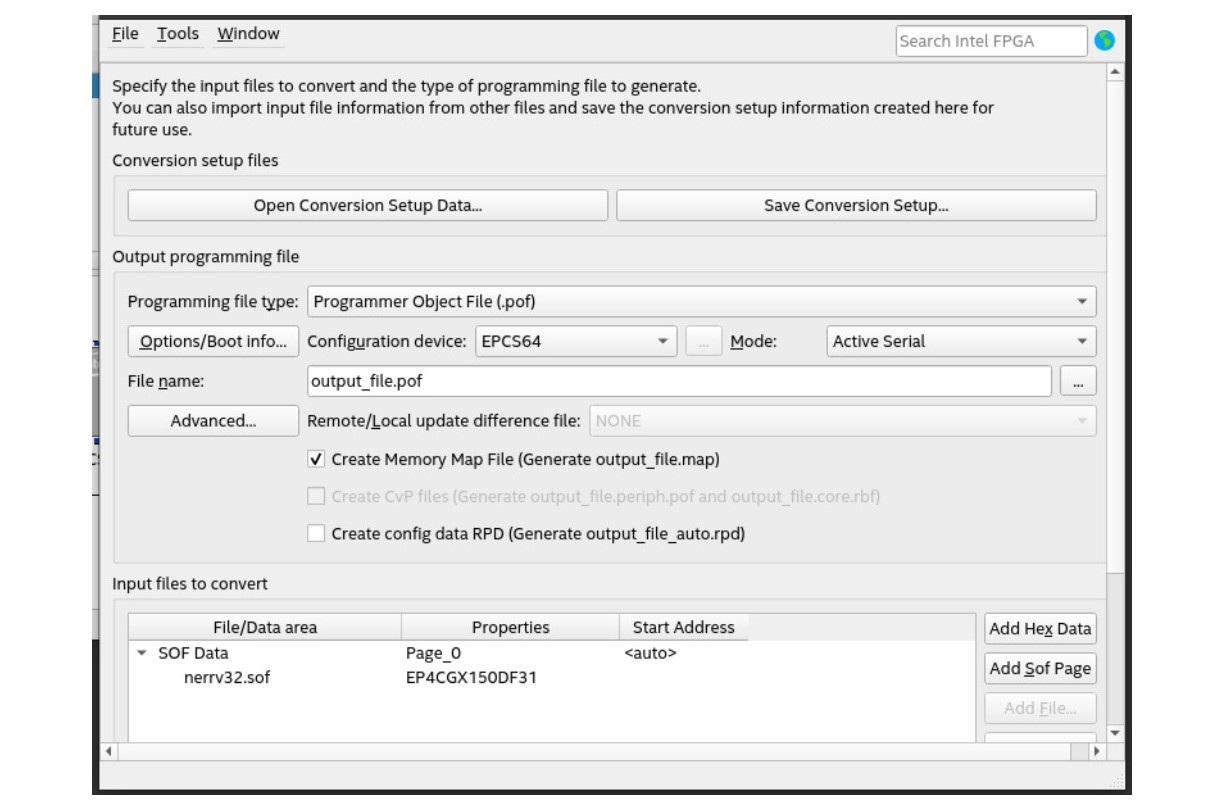
\includegraphics[width= 1\textwidth]{figures/chap2/fpga1.jpg}
                    \caption{\label{f1} Convert Programming Files Tool.}
                \end{center}
            \end{figure}
            
        2. On the FPGA switch to the recording mode (PROG) using the Programming Mode Switch shown in the Figure \ref{f2}.
        
            \begin{figure}[!ht]
                \begin{center}
                    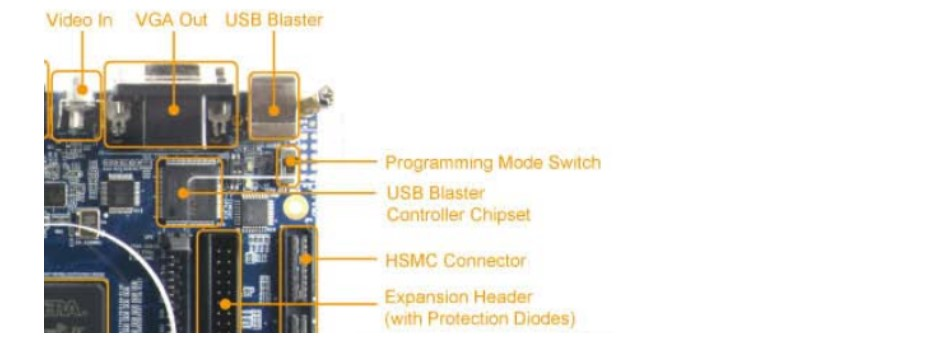
\includegraphics[width= 1\textwidth]{figures/chap2/fpga2.jpg}
                    \caption{\label{f2} Programming Switch Indication.}
                \end{center}
            \end{figure}
        
        3. Then open the Programmer via the path: Tools > Programmer.
            
            \begin{figure}[!ht]
                \begin{center}
                    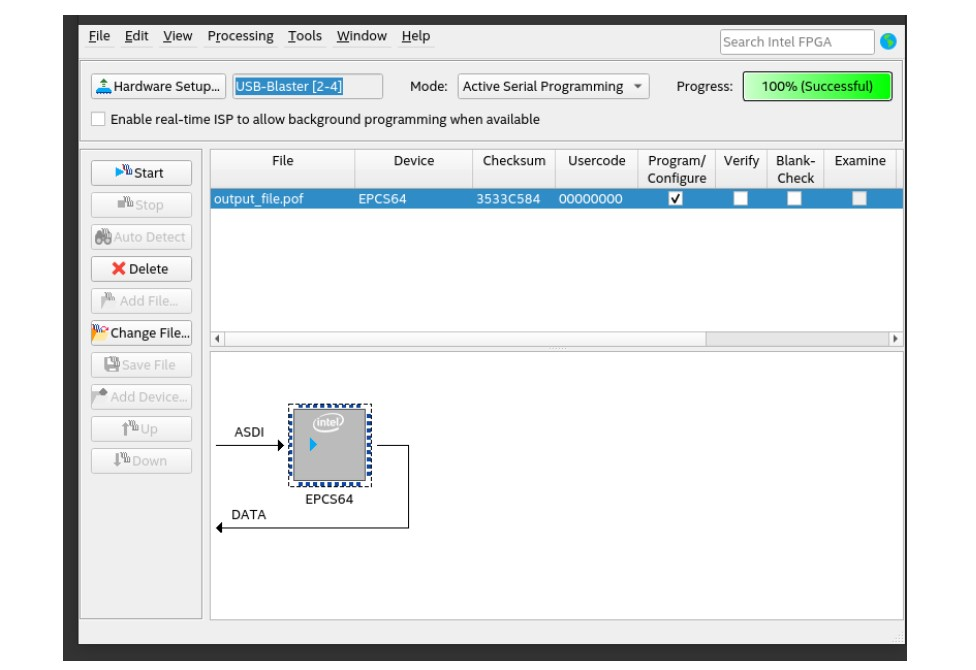
\includegraphics[width= 1\textwidth]{figures/chap2/fpga3.jpg}
                    \caption{\label{f3} Programmer Tool.}
                \end{center}
            \end{figure}
        
        4. Finally, Add Active Serial Programming, add the .pof file and click Start (Figure \ref{f3}). Before starting the FPGA, return the Programming Mode Switch to RUN mode.
        
%%%%%%%%%%%%%%%%%%%%%%%%%%%%%%%%%%%%%%%%%%%%%%%%%%%%%%%%%%%%%%%%%%%%%%%%%%%%%%%%%%%%%%%%%%%%%%%%%%%%%%%%%

\chapter{Compiling and executing your first program}
    https://www.overleaf.com/project/645bf9168256250a3c9f9d4f
    \section{Downloading and installing the toolchain}
    
        First, you should access \url{https://github.com/stnolting/riscv-gcc-prebuilt}, to download the most recent available toolchains (today, 21/05/2023, \textcolor{blue}{\textbf{rv32i-4.0.0}}). You should have now access to a .tar.gz file. Then, the next step, is to create the folder that the toolchain is going to be installed. You can open a terminal and type:
        
            \begin{lstlisting}[backgroundcolor = \color{lightgray}, language=bash]
                $ sudo mkdir /opt/riscv
            \end{lstlisting}
        
        Now, you need to navigate to the folder where the .tar.gz file was downloaded, like:
        
            \begin{lstlisting}[backgroundcolor = \color{lightgray}, language=bash]
                $ cd Downloads/
            \end{lstlisting}
            
        And then you have to extract the .tar.gz file to the folder previously created:
        
            \begin{lstlisting}[backgroundcolor = \color{lightgray}, language=bash]
                $ sudo tar -xzf <toolchain_version>.tar.gz -C /opt/riscv/
            \end{lstlisting}
            
        Finally, you should add the toolchain's bin folder to your system's PATH environment variable. You can open the .bashrc file:
        
            \begin{lstlisting}[backgroundcolor = \color{lightgray}, language=bash]
                $ sudo nano .bashrc
            \end{lstlisting}
            
        And then add the following line in the end of the .bashrc file:
        
            \begin{lstlisting}[backgroundcolor = \color{lightgray}, language=bash]
                export PATH="/opt/riscv/bin:$PATH"
            \end{lstlisting}
            
        To make sure everything works fine, navigate to the folder with the aplication examples and execute the following command:
        
            \begin{lstlisting}[backgroundcolor = \color{lightgray}, language=bash]
                $ make check
            \end{lstlisting}
        
        If everything is working fine you should se an "\textbf{OK}" appearing at the end, like in the \autoref{fig:successful_check}.
        
            \begin{figure}[!ht]
                \begin{center}
                    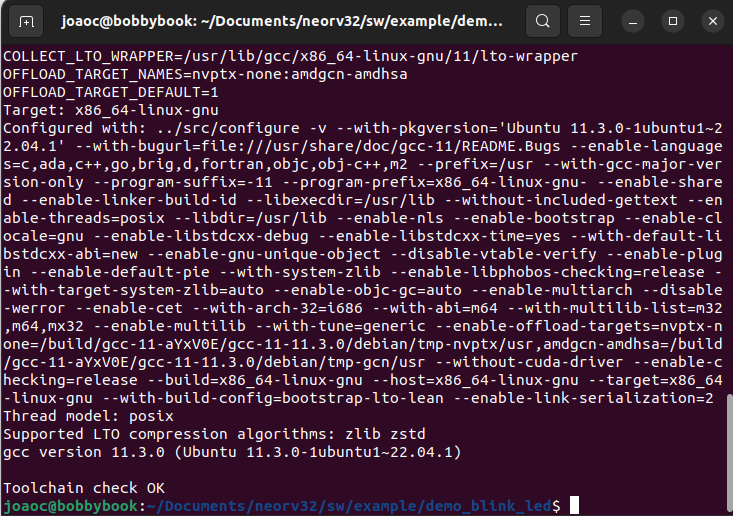
\includegraphics[width= 0.6\textwidth]{figures/successful_check.png}
                    \caption{Indication that the installation was successful.}
                    \label{fig:successful_check}
                \end{center}
            \end{figure}
    
        \subsection{Some important commands}
        
        Now that the toolchain was installed, you should know some commands to generate the .hex, .bin, .vdh, as well as other types of files. As you can see in \autoref{fig:toolchain_commands}, you could use \texttt{\hl{hex}} to generate the .hex file, which represents the machine language. You could use, for instance, the \texttt{\hl{image}} to generate the .vhd file, which is used to generate the \textit{neor32\_application\_image.vhd} that stores the main program that will run in the microprocessor. 
        
        
        \begin{figure}[!ht]
            \begin{center}
                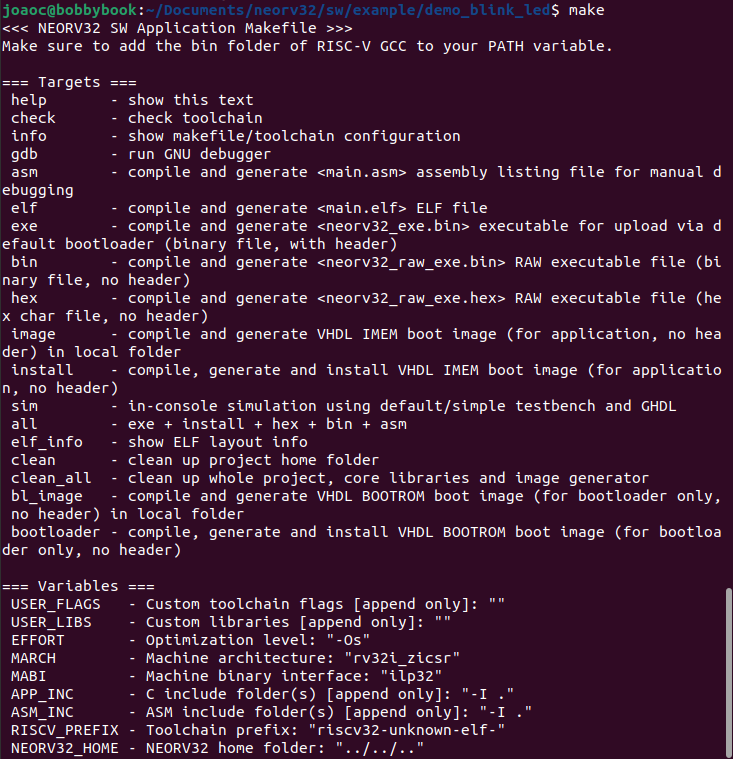
\includegraphics[width= 0.6\textwidth]{figures/toolchain_commands.png}
                \caption{Some useful commands to use.}
                \label{fig:toolchain_commands}
            \end{center}
        \end{figure}
        
    \section{Flash the program into FPGA Board using bootloader}
    
        In Linux, you should install a terminal emulator, like Minicom, Cutecom or similar:
        
            \begin{lstlisting}[backgroundcolor = \color{lightgray}, language=bash]
                $ sudo apt install cutecom
            \end{lstlisting}
        
        Then the software should be configured like in \autoref{fig:cutecom_configuration}.  With the FPGA previously programmed with the base of the NEORV32, you should see the status LED starts blinking and the bootloader intro screen appearing in your console, like:
        
            \begin{lstlisting}[backgroundcolor = \color{lightgray}, language=bash]
            
                << NEORV32 Bootloader >>
            
                BLDV: Mar  7 2023
                HWV:  0x01080107
                CID:  0x00000000
                CLK:  0x05f5e100
                MISA: 0x40901106
                XISA: 0xc0000fab
                SOC:  0xffff402f
                IMEM: 0x00008000 bytes @0x00000000
                DMEM: 0x00002000 bytes @0x80000000
            
                Autoboot in 8s. Press any key to abort.
            
            \end{lstlisting}
            
            \begin{figure}[!ht]
                \begin{center}
                    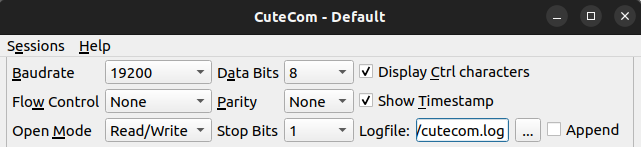
\includegraphics[width= 0.6\textwidth]{figures/cutecom_configuration.png}
                    \caption{Cutecom configuration.}
                    \label{fig:cutecom_configuration}
                \end{center}
            \end{figure}
            
        Now you can press any key to abort the automatic boot sequence and to start the actual bootloader user interface console. You then will have access to some commands, like:
        
            \begin{lstlisting}[backgroundcolor = \color{lightgray}, language=bash]
            
                Available CMDs:
                h: Help
                r: Restart
                u: Upload
                s: Store to flash
                l: Load from flash
                x: Boot from flash (XIP)
                e: Execute
                 
            \end{lstlisting}
        
        You can now upload the .bin file to execute it in the NEORV32. It will wait you to send the .bin file, so click on the \textit{send file} option to select the correct file. Finally, you can execute the program.
        
    \section{Flash the program into FPGA board directly}
        
        To generate an .vhd file for the IMEM that contains the actual application, run the \texttt{\hl{image}} inside the folder of your application. For instance, you could use any application from the NEORV32's examples folder, like neorv32-setup/sw/exmaple/demo\_blink\_led:
        
            \begin{lstlisting}[backgroundcolor = \color{lightgray}, language=bash]
                $ make clean_all image
            \end{lstlisting}
        
        This command will create the \textit{neorv32\_application\_image.vhd} file, that you can then add to the project's folder. If you are using Quartus II, you could replace the current application file or add it to the project if don't exists already.